\documentclass[11pt]{article}
\newcommand{\E}{\text{E}}
\usepackage{fullpage, amsmath, amsthm, graphicx, cite}

\setlength{\parindent}{0pt}
\newtheorem{thm}{Theorem}
\newtheorem{lem}[thm]{Lemma}
\newtheorem{prop}[thm]{Proposition}
\newtheorem*{cor}{Corollary}
\newtheorem*{rem}{Remark}
\newcommand{\vs}{\vspace{0.2cm}}
\begin{document}
\title{The Graph Recommendation Problem}
\author{Arda Antikacioglu, R. Ravi, Srinath Sridhar}
\maketitle
\section{Introduction}
As the amount of data a service collects and indexes increases, the
problem of surfacing relevant content arises and may companies face
this challenge today. Netflix needs to recommend similar movies,
Amazon and Bloomreach need to recommend similar products, Facebook
needs to recommend pages or friends. This recommendation problem is
hard to solve and often critical to the success of these services. For
example, when a user signs up for the first time, Facebook needs to
recommend them to as many people relevant as possible very quickly
because if a user does not need reach a certain friend count, his the
probability of retaining that user decreases rapidly. Similarly,
Amazon may want to surface an undersold product on more commonly
visited product pages, but the revenue gain will not be significant
enough unless a certain number of pages recommend the said
product. What makes this problem difficult is that you can only show
so many recommendations in high value spots without overwhelming the
user. So the number of recommendations a high traffic user or product
can make is limited, and these need to be allocated efficiently. This
motivates modeling the problem as a an optimization problem on graphs
as follows. \vs

We let $L$ and $R$ be sets of products or users. We model the
relationship between these sets of products or users by a bipartite
graph $G=(L,R,E)$ where there is an edge between between a $u\in L$
and $v\in R$ if they are related in some way. Our goal is to find
a subgraph $H\subseteq G$ such that $\deg_{H}(u) \leq c$ for all $u\in
L$ and the number of vertices $u\in L$ with $\deg_{G}(u) \geq
a$ is maximized. We will call this problem the $(c,a)$-graph
recommendation problem.\vs

This problem can capture all the examples described above. In the case
of Netflix $L$ is a set of movies and $R$ is a set of users. In the
case of Facebook $L$ is a set of active users and $R$ is a set of new
users who need friends. In Amazon and Bloomreach's case $L$ is a set
of high traffic/revenue products and $R$ is a set of products whose
exposure we seek to increase. \vs

There are special cases of the graph recommendation problem that can
be solved to optimality in polynomial time. In particular if $a=1$
then the problem is simply a maximum cardinality $b$-matching
problem. However, implementing the algorithms that solve $b$-matchings
such as the blossom algorithm in general graphs is tricky as they
involve a good deal of bookkeeping. Furthermore they take $O(v^{2.5})$
time at best and are memory-intensive. With web-scale sizes of the
problems encountered in practice, any solution that requires
superlinear time is unlikely to be practical. In this paper we
develop several linear time algorithms that operate locally and
therefore use very little memory, but still output solutions
that are near optimal in the average-case and worst case.

\section{Summary of Results}
Our main contributions are the following:
\begin{enumerate}

\item We describe several general models such as the Hierarchical Tree
  Model and the Cartesian Product Model which describe how graph
  recommendation subgraphs arise probabilistically.

\item For each of these models, we describe a simple randomized linear
  time algorithm that solves the graph recommendation problem to near
  optimality in expectation.

\item We also show that a simple linear time greedy algorithm can
  approximate the problem to a constant factor in the worst case.

\item We prove that optimal recommendation subgraphs that satisfy the
  most trivial upper bounds exist with high probability even in random
  bipartite graphs with logarithmic average degree.

\item We show that the models described in the problem can describe
  real-life recommendation subgraphs and that the random sampling
  algorithms we describe find near optimal solutions to the graph
  recommendation problem.

\end{enumerate}

\section{Models}
We describe four different models that can generate recommendation
graphs. The first model we describe is called the {\em fixed degree
model}, which is analyzed in Section \ref{fixed-degree}. In this
model, every $u\in R$ is related to a fixed number of uniformly
randomly chosen adjecent vertices $v\in R$. This model is interesting
not for its expressive power but because of its simplicity.  It is
easy to analyze and also motivates the analysis of richer models.

In Section \ref{weighted}, we generalize the fixed degree model to a
model where the graph is fixed and the edges can weights. In Section
\ref{hierarchy}, we analyze the {\em hierarchical tree model} which
aims to model recommendation trees that arise from relationships in a
product hierarchy. Finally, in Section~\ref{cartesian} we study the 
{\em cartesian product model} which aims to model recommendation 
graphs which arise from combining the relevancy advice of several 
different algorithms.

\section{Results}
\subsection{Fixed Degree Model}
\label{fixed-degree}

In this model, we assume that a bipartite graph $G=(L,R,E)$ is
generated probabilistically by the following procedure. Each
vertex $v\in L$, uniformly samples a set of $d$ neighbors
from $R$. For convenience let $|L|=l$, $|R|=r$ and $k=l/r$. From
$G$, we sample a subgraph $H$ where for each vertex $u\in L$ a set of
$c$ neighbors are sampled uniformly from set of incident vertices. The
following theorem derives a lower bound on the expected size $S$ of the
number $v\in R$ such that $\deg_H(v) \geq 1$.

\begin{thm}
Suppose that $G=(L,R,E)$ and $H\subseteq$ is generated as above. Then
\[ \E[S] \geq r(1-\exp(-ck))\]
where the expectation is over the random sampling of $G$ and $H$.
\end{thm}
\begin{proof}
For each $v\in R$ let $X_v$ be the indicator variable for the event
that $\deg_H(v) \geq 1$. Note that since for each vertex $u\in L$, $H$
uniformly samples from a uniformly sampled set of neighbors, we can
think $H$ as being generated by the same process that generated $G$,
but with $d$ replaced with $c$. Now for a specific vertex $u \in R$,
the probability that it has no incident edges is 
$\left(1-\frac{1}{r}\right)^c$. Since the selection of neighbors for each 
vertex in $L$ is independent, it follows that that:
\[ \Pr[X_v=0] = \left(1-\frac{1}{r}\right)^{cl} \leq \exp\left(-c \cdot \frac{l}{r}\right) = \exp(-ck) \]
Note that $S = \sum_{v\in R} X_v$. Applying linearity of expectation, we get
\[ \E[S] = \sum_{v\in V} \E[X_v] \geq r(1-\exp(-ck))\]
\end{proof}

While this shows a lower bound in absolute terms, we must compare it to the best possible solution {\em OPT}. The follow theorem proves the approximation ratio to {\em OPT}.

\begin{thm}
The above sampling algorithm gives a $1-1/e$ factor approximation to the $(c,1)$-graph recommendation problem in expectation
\end{thm}
\begin{proof}
The size of the optimal solution is bounded above by both the number
of edges in the graph and the number of vertices in $R$. The former of
these is $cl=ckr$ and the latter is $r$, which shows that $OPT \leq
r\max(ck,1)$. Therefore, by simple case analysis the approximation ratio in
expectation is at least
\[ \frac{1-\exp(-ck)}{\min(ck,1)} \geq 1-\frac{1}{e} \]
\end{proof}

However in reality, the approximation obtained by this sampling
approach can be much better for certain values of $ck$. In particular,
if $ck>1$, then the approximation ratio is $1-\exp(-ck)$, which
approaches 1 as $ck\to\infty$. In particular, if $ck=3$, then the
solution will be at least 95\% as good as the optimal solution even
with our trivial bounds. Similarly, when $ck<1$, the approximation
ratio is $(1-\exp(-ck))/ck$ which also approaches 1 as $ck\to 0$. In
particular, if $ck=0.1$ then the solution will be at 95\% as good as
the optimal solution. The case when $ck=1$ therefore represents the
worst case outcome for this model where we only guarantee 63\%
optimality. The graph below shows the approximation ratio as a
function of $ck$.

\begin{figure}[h]
\centering
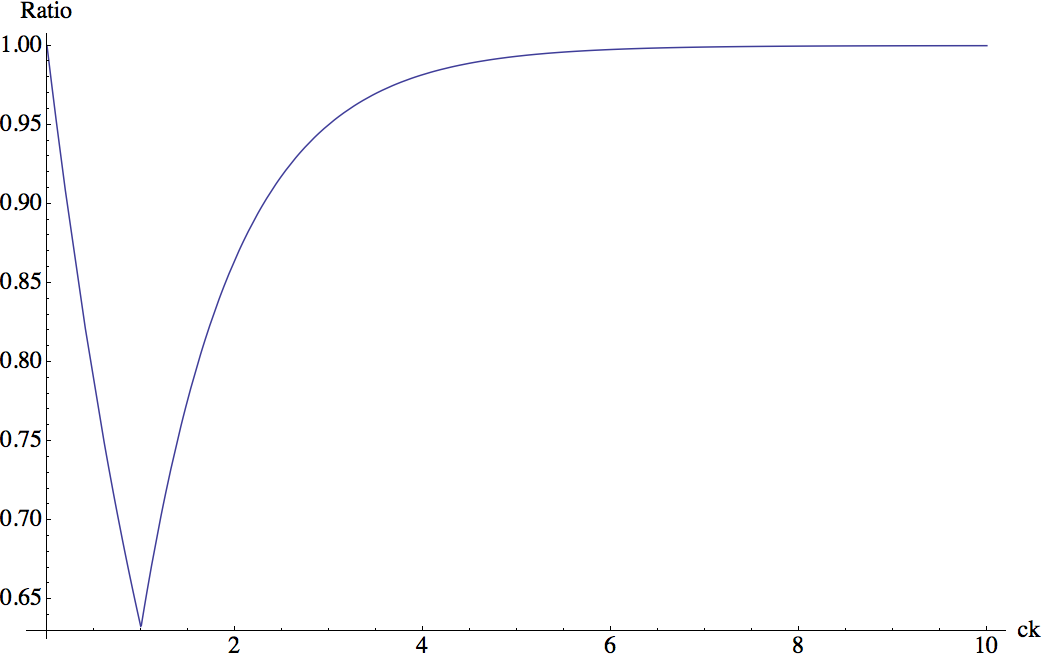
\includegraphics[width=10cm]{Sri_Original.png}
\caption{Approximation Ratio as a function of $ck$ }
\end{figure}

Now suppose that $G$ is generated and $H$ is sampled using the same
processes as described above. In the next theorem, we extend the above
bounds to the $(c,a)$-graph recommendation problem where $a>1$. 
%In particular if we set $a=1$, we will obtained the estimate from the original analysis.

\begin{thm}
Let $S$ be the random variable denoting the number of vertices $v \in R$ such that $\deg_{H}(v)\geq a$. Then
\[ \emph{\E}[S] \geq r\left(1-e^{-ck+\frac{a-1}{r}}\frac{(ck)^a-1}{ck-1}\right)  \]
where the expectation is over the randomness of $G$ and $H$.
\end{thm}

\begin{proof}
Let $X_{uv}$ be the indicator variable of the event that the edge $uv$
(note that $u\in L$ and $v\in R$) is in the subgraph that we picked
and set $X_{v} = \sum_{u\in U} X_{uv}$ so that $X_{v}$ represents the
random degree of the vertex $v$ in our subgraph. Because our algorithm
uniformly subsamples a uniformly random selection of edges, we can
assume that$H$ was generated the same way as $G$ but sampled $c$
instead of $d$ edges for each vertex $u\in L$. So $X_{uv}$ is a
bernoulli random variable. Using the trivial bound $\binom{n}{i}
\leq n^i$ on binomial coefficients we get:
\begin{align*}
      \Pr[X_v < a]
&=    \sum_{i=0}^{a-1} \binom{cl}{i} \left(1-\frac{1}{m}\right)^{cl-i}\left(\frac{1}{r}\right)^i \\
&\leq \sum_{i=0}^{a-1} \left(\frac{cl}{r}\right)^i\left(1-\frac{1}{r}\right)^{cl-i} \\
&=    \left(1-\frac{1}{r}\right)^{cl-(a-1)}\sum_{i=0}^{a-1} (ck)^i \\
&\leq \left(1-\frac{1}{r}\right)^{cl-(a-1)}\frac{(ck)^a-1}{ck-1} \\
&\leq e^{-ck+\frac{a-1}{r}} \frac{(ck)^a-1}{ck-1}
\end{align*}


Letting $Y_v = \left[X_v \geq a\right]$, we now see that

\[ \E[S] = \E\left[\sum_{v\in R} Y_v\right] \geq r\left(1-e^{-ck+\frac{a-1}{r}} \frac{(ck)^a-1}{ck-1}\right) \]
\end{proof}

Now, we can perform a similar analysis as in the previous section. In
particular, if $ck>a$, then the problem is easy on average though we
need $ck$ to get larger than before to be close to optimal. This
is in comparison to the trivial estimate of $m$. For a fixed $a$, a
random solution gets better as $ck$ increases because the decrease in
$e^{-ck}$ more than compensates for the polynomial in $ck$ next to
it. However, if $ck<a$, we need to use the trivial estimate of
$ckr/a$, and the analysis from the previous section does not extend
here. \\

In both this section and the previous one, $ck$ is the average degree
of a vertex $v\in R$ in our chosen subgraph. Basically, what the
original analysis said is that if $ck>1$, then the sampling algorithm
will probably cover every vertex in $R$ since the expected degree of
each vertex is large. On the other hand if $ck$ is small ($ck < 1$)
then the best possible solution is obtained when none of the vertices
in $R$ has degree greater than 1. If $ck<1$, then we do not cover very
many vertices in $R$, but we also do not cover many vertices more than
once. Since the optimal solution in this case was correspondingly low,
our solution was good in the $a=1$ case. However, when $a<1$, the fact
that our edges are well-dispersed only hurts our solution because we
need to concentrate the edges on particular $v\in R$ that will
count. The following table shows how large $ck$ needs to be for the
solution to be 95\% optimal for different values of $a$:

\begin{figure}[h]
  \centering
  \begin{tabular}{ |c|c|c|c|c|c| }
    \hline
    $a$ & 1 & 2 & 3 & 4 & 5 \\ \hline
    $ck$ & 3.00 & 4.74 & 7.05 & 10.01 & 13.48 \\
    \hline
  \end{tabular}
  \caption{The required $ck$ to obtain 95\% optimality}
\end{figure}

\subsection{Hierarchical Tree Model}
\label{hierarchy}
In this section we explore the hierarchical tree model. We will assume
that we are given a bipartite graph $G=(L,R,E)$. The vertex sets $L$
and $R$ are the leaf sets of two full binary trees $T_L$ and $T_R$ of
depth $D$ where there is a one-to-one correspondence between the
subtrees of these two trees. We also assume that each branching in
both $T_L$ and $T_R$ splits the nodes evenly into the two
subtrees. By abuse of notation, we will use a subtree and its leaf set
interchangeably. The trees are fixed in advance, but $G$ is generated
probabilistically according to the following procedure. Let $u\in L$
and $T_L^0, \ldots T^{D-1}_L$ be the subtrees it belongs at depths
$0,\ldots, D-1$. Also, let $T_R^0,\ldots, T_R^{D-1}$ be the subtrees
on the right that correspond to these trees on the left. We let $u$
make an edge to $d_{D-1}$ of the vertices in $T_{R}^{D-1}$, $d_{D-2}$
edges to the vertices in $T_{R}^{D-1} \backslash T_{R}^{D-2}$ and so
on. Each vertex is chosen with uniform probability and we let $d =
d_{0} + \ldots + d_{D-1}$.\vs

\begin{figure}[h]
\centering
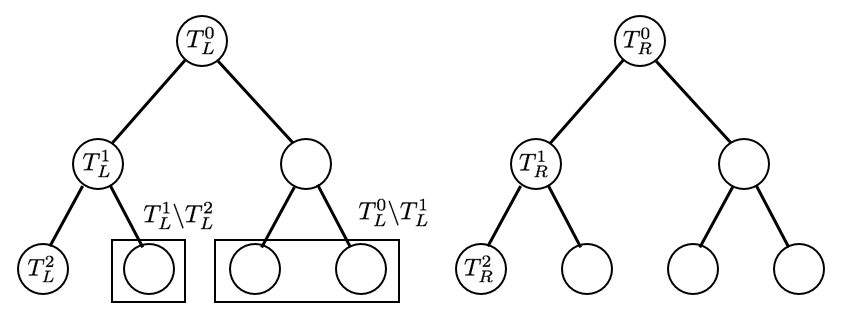
\includegraphics[width=0.6\textwidth]{hierarchy_tree.png}
\begin{minipage}[h]{0.7\textwidth}
\caption{This diagram shows the notation we use for this model and the 1-to-1 correspondance of subtrees}
\end{minipage}
\end{figure}

Our goal now is to find a $b-$matching in this graph that is close to
optimal in expectation. That is, our degree upper bound on vertices in
$L$ is $c$ and the degree lower bound on vertices in $L$ is 1. Let $c
= c_0 + \ldots + c_{D-1}$ where the fractions $d_{i}/c_{i}$ are all
equal to some constant $k$. For simplicity assume that $k$ is an
integer. To combine the analysis of the randomness of the algorithm
and the randomness of the graph, the algorithm will pick $c_{i}$ edges
uniformly from among the $d_{i}$ edges going to each level of the
subtree. This enables us to think of the subgraph our algorithm
outputs as being generated by the graph generation process, but with
fewer neighbors selected for each as in the previous sections. With
this model and parameters in place, we can prove the following
theorem.\

\begin{thm}
Let $S$ be the subset of edges $v\in R$ such that $\deg_H(v) \geq 1$. Then
\[ \E[S] \geq r(1-\exp(-ck)) \]
where the expectation is taken over $G$ and $H$.
\end{thm}

\begin{proof}
Let $v\in R$ and let $T_L^{D-1}, T_L^{D-2}\backslash T_L^{D-1},
\ldots, T_L^0\backslash T_L^1$ be the sets it can take edges
from. Since $T_L$ and $T_R$ split perfectly evenly at each node the
vertices in these sets will be choosing from $r_{D-1}, r_{D-1},
r_{D-2},\ldots, r_{1}$ vertices in $R$ for neighbors respectively,
where $r_i$ is the size of subtree of the right tree rooted at depth
$i$. Furthermore, each of these sets described above have size
$l_{D-1}, l_{D-1}, l_{D-2}, \ldots, l_{1}$ respectively, where $l_i$
is the size of a subtree of $T_L$ rooted at depth $i$. It follows that
the probability that $v$ does not receive any edges at all is at most

\begin{align*}
	      \Pr[\lnot X_v] 
	&=    \left(1-\frac{1}{r_{D-1}}\right)^{c_0l_{D-1}}\prod_{i=1}^{D-1}\left(1 - \frac{1}{r_i}\right)^{c_{D-i} l_i} \\
	&\leq \exp\left(-\frac{l_{D-1}}{r_{D-1}}c_0\right)\prod_{i=1}^{D-1} \exp\left(\frac{l_i}{r_i}c_{D-i}\right) \\
	&=    \exp\left(-(c_0 + \ldots + c_{D-1})k\right) \\
	&=    \exp(-ck)
\end{align*}

Since this is an indicator variable, it follows that 
\[ \E[S] = \E\left[\sum_{v \in R} X_v \right] \geq r \left(1-\exp(-ck)\right) \]
\end{proof}

Note that this is the same result as we obtained for the fixed degree
model in Section \ref{fixed-degree}. In fact, the approximation
guarantees when $ck \ll 1$ or $ck \gg 1$ hold exactly as before.\vs

The sampling of $H$ can be done algorithmically because we separated
out the edge generation process at a given depth from the edge
generation process at deeper subtrees. There is no ambiguity as to why
an edge is in the underlying graph. That is, if we superimpose $T_L$
and $T_R$, then an edge between $u_l\in L$ and $v_r\in R$ must have
come from an edge generated at the lowest common ancestor of $u_l$ and
$v_r$. So the algorithm can actually sample intelligently and in the
same way that the graph was generated in the first place. Also note
that we do not have to assume that the trees $T_L$ and $T_R$ are
binary. We only need the trees to be regular and evenly divided at
each vertex since the proof only relies on the proportions of the
sizes of the subtrees in $T_L$ and $T_R$.


\subsection{Cartesian Product Model}
\label{cartesian}
We can extend the analysis in Section \ref{fixed-degree} in a way
orthogonal to the hierarchical tree model as follows. We assume that
$L$ has been partitioned into $t$ subsets $L_1,\ldots, L_t$ and
that $R$ has been partitioned into $t'$ subsets $R_1,\ldots,
R_{t'}$. For convenience, we let $|L_i| = l_i$ and $|R_i|=r_i$. Given
this suppose that for each $1\leq i\leq t$ and each $1\leq j\leq t'$,
$G[L_i, R_j]$ is an instance of the Fixed Degree Model with
$d=d_{ij}$. We assume that for all $i$, we have $\sum_{j=1}^{t'}
d_{ij} = d$ for some fixed $d$. Also assume that we have fixed in
advance $c_{ij}$ for each $1\leq i\leq t$ and $1\leq j\leq t'$ that
satisfy $\sum_{j=1}^{t'} c_{ij} = c$ for all $i$ for some fixed $c$.
To sample $H$ from $G$, we sample $c_{ij}$ neighbors for each 
$u_i\in L_i$ from $R_i$. Letting $S$ be the set of vertices in 
$v\in R$ that satisfy $\deg_H(v)\geq 1$, we can show the following:

\begin{thm}
With $S$, $G$ and $H$ defined as above, we have
\[ \E[S] \geq r - \sum_{j=1}^{t'} r_j \exp\left(-\sum_{i=1}^t c_{ij} \frac{l_i}{r_j}\right)\]
where the expectation is over $G$ and $H$.
\end{thm}
\begin{proof}
Let $v_j \in R_j$ be an arbitrary vertex and let $X_{v_j}$ be the
indicator variable for the event that $\deg_H(v_i) \geq 1$. The
probability that none of the neighbors of some $u_i\in R_i$ is $v_j$
is exactly $(1-\frac{1}{r_j})^{c_{ij}}$. It follows that the
probability that the degree of $v_j$ in the subgraph $H[L_i,R_j]$ is 0
is at most $(1-\frac{1}{r_j})^{c_{ij}l_i}$. Considering this
probability over all $R_j$ gives us:
\[ \Pr[X_{v_i} = 0] = \prod_{i=1}^{t} \left(1-\frac{1}{r_j}\right)^{c_{ij} l_i} \leq \exp\left(-\sum_{i=1}^t c_{ij} \frac{l_i}{r_j}\right)\]

By linearity of expectation $\E[S] = \sum_{i=1}^{t'} r_i \E[X_{v_i}]$,
so it follows that
\[ \E[S] \geq \sum_{j=1}^{t'} r_j \left(1-\exp\left(-\sum_{i=1}^t c_{ij} \frac{l_i}{r_j}\right)\right) = r - \sum_{j=1}^{t'} r_j \exp\left(-\sum_{i=1}^t c_{ij} \frac{l_i}{r_j}\right)\]
\end{proof}

This model is interesting because it can capture a broader set of
recommendation subgraphs than the fixed degree model. However, it is
difficult to estimate how good a solution will be without knowing
the sizes of the sets in the partitions. However, we can note that we
obtain the approximation guarantee of $(1-\exp(-ck))$ provided that
$l_i/r_j = k$ for all $i$ and $j$ where $k$ is some fixed
constant. Another interesting point about this model and the algorithm
we described for sampling $H$ is that we are free to set the $c_{ij}$
as we see fit. In particular, $c_{ij}$ can be chosen to maximize the
approximation guarantee in expectation we obtained above using
gradient descent or some other first order method prior to running the
recommendation algorithm to increases the quality of the solution.


\subsection{Weighted Model}
\label{weighted}
The fixed degree model of Section \ref{fixed-degree} is a simple and
convenient model, but the assumption that all recommendations hold the
same weight is unrealistic. This motivates fixing the graph to be the
complete bipartite graph $K_{l,r}$, and giving the edges i.i.d weights
with mean $\mu$. We modify the objective function accordingly, so that
we count only the vertices in $R$ which have weight $\geq 1$. If we
assume that $ck\mu \geq 1+\epsilon$ for some $\epsilon > 0$, then 
naive the solution sampling solution we outlined in Section \ref{fixed-degree}
still performs exceptionally well. Letting $S$ be the size of the 
solution produced by this algorithm we have:

\begin{thm}
Let $G=K_{l,r}$ be a bipartite graph where the edges have i.i.d. weights and come from a distribution with mean $\mu$ that is supported on $[0,b]$. If the algorithm from Section \ref{fixed-degree} is used to sample a subgraph $H$ from $G$, then
\[ \E[S] = \sum_{v\in R} \E[X_v] = r\left(1-\exp\left(-\frac{2l\epsilon^2}{b^2}\right)\right) \]
\end{thm}

\begin{proof}
For each edge $uv\in G$, let $W_{uv}$ be its random weight, $Y_{uv}$ be
the indicator for the event $uv\in H$ and define $X_{uv} = Y_{uv}
W_{uv}$. Since weights and edges are sampled by independent processes,
we have $\E[X_{uv}] = \E[W_{uv}]\E[Y_{uv}]$ for all edges. Since $c$
edges out of $r$ are picked for each vertex, $\E[Y_{uv}] = \frac{c}{r}$
, so $\E[X_{uv}] = \frac{c}{r}\mu$. Therefore, the expected weight
coming into a vertex $v\in R$ would be 

\[ \E[X_v] = \sum_{u\in L} \E[X_{uv}] = \frac{cl\mu}{r} = ck\mu\]

However, $X_{uv}$ for each $u$ are i.i.d random variables. Since by
assumption $ck\mu = 1+\epsilon$, by a Hoeffding bound we can obtain:

\[ \Pr[X_v \leq 1] = \Pr[X_v - \E[X_v] \geq \epsilon] \leq \exp\left(-\frac{2l\epsilon^2}{b^2}\right) \]

By linearity of expectation we can now get the result in the theorem

\[ \E[S] = \sum_{v\in R} \E[X_v] = r\left(1-\exp\left(-\frac{2l\epsilon^2}{b^2}\right)\right) \]
\end{proof}

There are two things to note about this variant. The first is that
since the variables $X_v$ are negatively correlated, our results in
\ref{worst-vs-avg} can be readily extended to the results of this
section. The second is that the condition that $W_{uv}$ are i.i.d
is not necessary to obtain the full effect of the analysis. Indeed,
the only place in the proof where the fact that $W_{uv}$ are i.i.d
is when we argued that $X_{uv}$ is large with high probability by a
Hoeffding bound. For the bound to apply, it's sufficient to assume
that $W_{uv}$ for all $v$ are independent. In particular, it's 
possible that $W_{uv}$ for all $u$ are inter-dependent. This allows
us to assume an weight distribution that depends on the strength of 
the recommender and the relevance of the recommendation separately.


\section{Worst-Case Approximation}
The results in the previous section concentrated on producing nearly
optimal solutions in expectation. In this section, we will show that
it is possible to obtain good solutions regardless of the model that
generated the recommendation subgraph. As usual we let $G=(L,R,E)$ be a
bipartite graph on which we would like to solve the (c,a)-graph
recommendation problem and consider the following greedy
algorithm. Consider each vertex in $R$ in some arbitrary order and if
there is some $v \in R$ that has $a$ neighbors in $L$ all of which
have degree $< c$, add the edges to these neighbors to $H$. If there
are any ties about the nodes to be picked either in the selection of
$v$ or its neighbors, we can break ties arbitrarily. This algorithm
has the following approximation guarantee

\begin{thm}
The greedy algorithm described above achieves a $1/(a+1)$-approximation ratio.
\end{thm}
\begin{proof}
Let $R_{GREEDY}, R_{OPT}\subseteq R$ be the set of vertices that have
degree $\geq a$ in the greedy and optimal solutions respectively. Note
that any $v \in R_{OPT}$ along with neighbors $\{u_1,\ldots u_a\}$
forms a set of candidate edges that can be taken by the greedy
algorithm. So we can consider $R_{OPT}$ as a candidate pool for
$R_{GREEDY}$. Each move that the greedy algorithm makes might make
some of the candidates infeasible, but as long as the candidate pool
is not depleted, the greedy algorithm can continue adding vertices to
its solution. Each time the greedy algorithm claims some vertex $v\in
R$ with edges to $\{u_1,\ldots, u_a\}$, we have obviously have to
remove $v$ from the candidate pool. If any $u_i$ was saturated
(i.e. had degree $c$) in the optimal solution, we would also need to
remove an arbitrary vertex $v_i\in R$ adjacent to $u_i$ in the optimal
solution. In other words, by using an edge of $u_i$, we force it to
not use an edge it used to some other $v_i$, which might cause the
degree of $v_i$ to go below $a$. (Note that the greedy algorithm does
not actually have to be aware of the structure of optimal solution for
this type of bookkeeping to go through.) Therefore, at each step of
the greedy algorithm, we have to remove at most $a+1$ vertices from
the candidate pool. Since our candidate pool has size $OPT$, the
greedy algorithm cannot stop before it has added $|OPT|/(a+1)$
vertices to the solution.
\end{proof}

\begin{figure}[h]
\centering
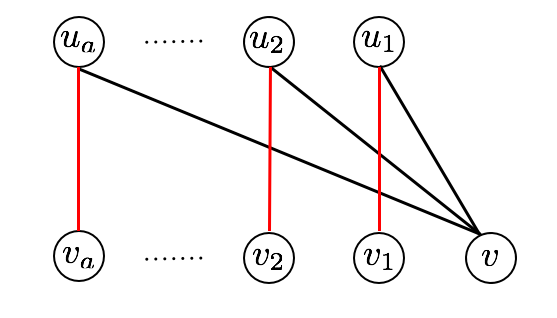
\includegraphics[width=.5\textwidth]{greedy.png}
\begin{minipage}[h]{.8\linewidth}
\caption{This diagram shows one step of the greedy algorithm. When $v$ claims edges to $u_1,\ldots, u_a$, it potentially removes $v_1,\ldots, v_a$ from the pool of candidates that are avaiable. The potentially invalidated edges are shown in red.}
\end{minipage}
\end{figure}

There are several things to note about this algorithm. The first is
that the solution the greedy algorithm outputs is dependent on the
order the vertices in $R$ are processes. It may be possible to improve
the expected approximation ratio by permuting these vertices randomly
before the algorithm runs. The second is that this approximation
guarantee is as good as we can expect. In particular, if we set $a=1$
then we obtain the familiar $1/2$-approximation for matchings. It
might be possible that some or even all the cases of the graph
recommendation problem admit $(1+\epsilon)$ approximations in
$O(n\cdot \text{polylog}(n))$ time, but this greedy algorithm likely
represents the best we can do with minimal effort. Finally, we can use
this worst case approximation algorithm to benchmark the random
sampling algorithms we described in the previous section.

\label{worst-vs-avg}
\section{Comparing the Worst-Case and Average-Case Approximations}
In this section, we show that the the results of Section
\ref{fixed-degree} that hold in expectation also hold in the worst
case with high probability using concentration bounds.

We can convert the expectation results to a lower bound that holds
with high probability in two ways. First, recall that Markov's
inequality states that for any non-negative random variable $X$ and
any $a\geq 1$, we have $\Pr[X \geq a\E[X]] \leq \frac{1}{a}$. We can
apply this to the random variable $r-S$ with $a=\frac{1}{2}$ to
obtain:

\begin{thm}
The random sampling algorithm produces a solution of size at least $r(1-2\exp(-ck))$ with probability at least $1/2$, 
\end{thm}

While this gives us a lower bound, we can do better using Chernoff
bounds. While Chernoff bounds are usually stated for independent
variables, the bound bound below holds for non-positively correlated
variables.

\begin{thm}
Let $X_1,\ldots, X_n$ be non-positively correlated variables. If $X=\sum_{i=1}^n X_i$, then for any $\delta\geq 0$
\[ Pr[X \geq (1+\delta)\E[X] ] \leq \left(\frac{e^\delta}{(1+\delta)^{1+\delta}}\right)^{\E[X]} \]
\end{thm}

Now note that the variables $1-X_v$ for each $v\in R$ are
non-positively correlated. In particular, if $N(v)$ and $N(v')$ are
disjoint, then $1-X_v$ and $1-X_{v'}$ are independent. Otherwise, $v$
not claiming any edges can only increase the probability that $v'$
gets an edge from any vertex $u\in N(v)\cap N(v')$, so the variables
would be negatively correlated. Setting $\delta\approx 1.39$ in the
theorem above now proves the following:

\begin{thm}
The random sampling algorithm produces a solution of size at least $r(1-2\exp(-ck))$ with probability at least $(e/4)^{r\exp(-ck)}$.
\end{thm}

That is, the probability of producing a constant factor approximation decreases exponentially with $r$.

With these high probability bounds in place, it is instructive to
compare the performance of the random sampling algorithm with that of
the $c=1$. With high probability, the approximation ratio of the
randomized algorithm is $(1-\exp(-ck))/(1-\exp(-dk))$ while the
approximation ratio of the greedy algorithm is always at least
$1/2$. In the following graphs $f\geq 1$ represents a value such that
$d=fc$ and we use the values $k=0.1$ and $k=0.2$ respectively since
the case that is practical for our purposes is when $l \ll r$. In the
graphs below, the red curve shows the approximation ratio for the
model used in Section \ref{fixed-degree} and the blue curve shows the
worst case approximation ratio described in section 5. As we would
expect, the sampling algorithm performs outperforms the greedy
algorithm significantly when $k$ and more importantly $c$ gets larger.

\begin{figure}[h]
\begin{minipage}[h]{0.45\linewidth}
\centering
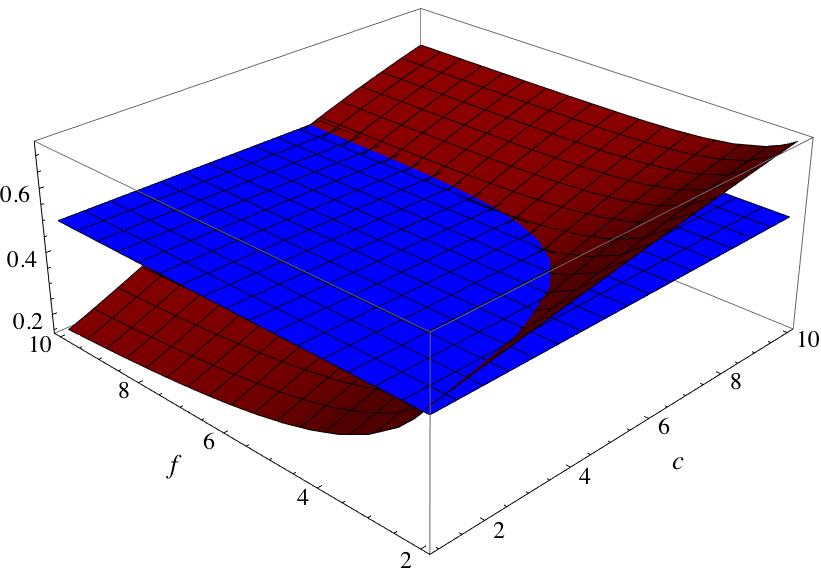
\includegraphics[width=\textwidth]{k=0_1.png}
\caption{Approximation ratios when $k$=0.1}
\end{minipage}
\hspace{0.5cm}
\begin{minipage}[h]{0.45\linewidth}
\centering
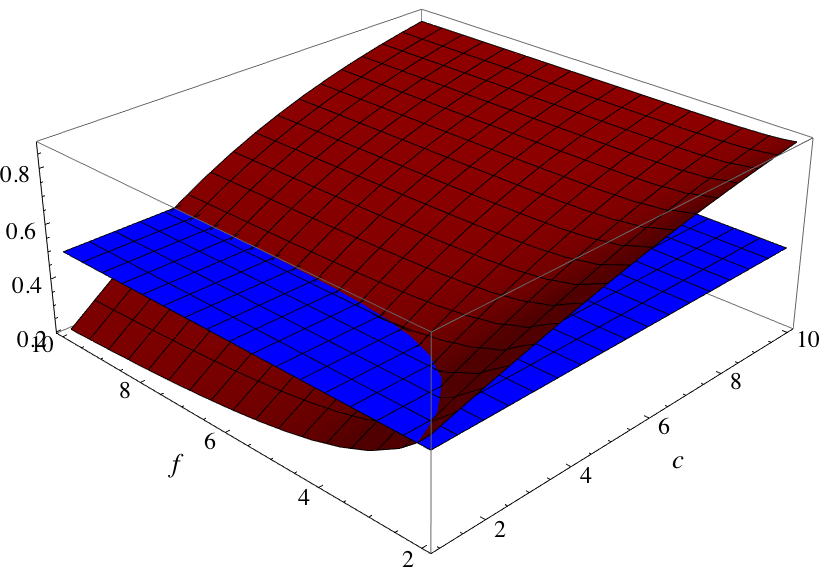
\includegraphics[width=\textwidth]{k=0_2.png}
\caption{Approximation ratios when $k$=0.2}
\end{minipage}
\end{figure}


\section{Existance of Optimal Recommendation Subgraphs}
Let $G=(L,R,E)$ be a bipartite graph. We define a \emph{perfect} $(c,a)$-recommendation on $G$ to be a subgraph $H$ such that $deg_H(u)\leq c$ for all $u\in L$ and $deg_H(v)=a$ for all $v\in R$. In this section we will prove a sufficient condition for perfect $(a,a)$-recommendation subgraphs to exist in a bipartite graph where edges are sampled uniformly and independently with probability $p$. Our result, hinges on the following characterization of optimal recommendation subgraphs due to Enomoto, Kano and Ota \cite{EKO}:

\begin{thm}
Let $G=(L,R,E)$ be a bipartite graph, $k=|L|/|R|$ and $\lambda = a - 1 + 1/c$. Then an optimal $(c,a)$-recommendation subgraph exists if 

\begin{itemize}
\item $a \leq ck$
\item for every set $S\subseteq R$ such that $|S| < n/\lambda$, $|N(S)| > \lambda|S|$
\item for every set $S\subseteq R$ such that $|S| \geq n/\lambda$, $N(S) = L$
\end{itemize}
\end{thm}
 
Note that in a perfect $(c,a)$-recommendation subgraph there are exactly $a|R|$ edges. Therefore, the first condition merely states that the number of vertices in $L$ must be high enough to support this many edges given that each of those vertices have degree at most $a$. The other two conditions state that any subset of vertices in $R$ must expand into $L$ by a factor of $\lambda$. The next theorem shows that this expansion property is satisfied with high probability if the edge selection probability is high enough. We will use this result first to prove a special case where $a=c$ and $|L|=|R|=n$. In order to this, we first need to prove a lemma.

\begin{lem}
Suppose that $G=(L,R,E)$ is a bipartite graph with $|L|=|R|=n$ that does not have a perfect $(a,a)$-recommendation subgraph. Then there exists a set $S\subseteq L$ or $S\subseteq R$ satisfying $|S|\leq n/(\lambda+1)$ and $|N(S)| < |S|\lambda$.
\end{lem}

\begin{proof}
First note that when $|L|=|R|$, a perfect $(a,a)$-recommendation subgraph assigns degree $a$ to each vertex in $R$ and degree at most $a$ to each vertex in $L$. In order for there to be the same number edges coming out of $L$ as there are out of $R$, the degree of every vertex such a recommendation subgraph needs to be $a$.\vs

This means that if a $(a,a)$-recommendation subgraph doesn't exists in $G$, then there doesn't exists on in $G$ when we flip the labels of $L$ and $R$. Applying Theorem 11, we now see that there must exists some $S$ that's either a subset of $L$ or $R$ that doesn't expand into a set $T$ that's of size at least $\lambda|S|$. We will assume without loss of generality that $S\subseteq L$ and consider the minimal such $S$ and let $|S|=nb$ for some constant fraction $b$. \vs

However, note that if there are no edges between $S$ and $R\backslash T$, then $N(R\backslash T) = L\backslash S$. Since we picked $S$ to be minimal in size, we must have $|S|\leq |R\backslash T|$ or equivalently, $nb \leq n -nb\lambda$. Rearranging this inequality shows that $b(\lambda+1) \leq 1$ or that $b\leq 1/(\lambda+1)$ as required.
\end{proof}

Using this lemma, we can prove the following theorem:

\begin{thm} 
Let $G=(L,R,E)$ be a bipartite graph with $|L|=|R|=n$ drawn from $G_{n,n,p}$. There exists some $c$ that only depends on $a$ such that if $p=c\ln(n)/n$, then $G$ has a perfect $(a,a)$-recommendation subgraph with probability 1 as $n\to\infty$.
\end{thm}

\begin{proof}
Let $\lambda = a - 1 + 1/a$. Using the lemma above, if $G$ does not have a perfect $(a,a)$-recommendation subgraph, then there must be a set $S$ such that $|S|\leq n/(\lambda+1)$ that's either contained in $R$ or $L$ that expands into a set $T$ of size less than $|S|\lambda$.

Therefore, we will consider all pairs of sets $S\subseteq R$ such that $|S|<n/2\lambda$ and $T\subseteq L$ such that $|T| = \lambda|S|$. If $N(S)\subseteq T$, then none of the at least $s(n-\lambda s)$ edges between $S$ and $L\backslash T$ can be present in $G$ (and similarly for $S\subseteq L$). By a union bound, this probability is at most: 

\begin{align*}
       \Pr\left[\bigvee_{\substack{|S|\leq n/(\lambda+1) \\ |T| = \lambda |S|}} \text{S fails to expand out of T}\right]
\leq&  2\sum_{s=1}^{n/(\lambda+1)} \binom{n}{s}\binom{n}{s\lambda}(1-p)^{s(n-s\lambda)} \\
\leq&  2\sum_{s=1}^{n/(\lambda+1)} \left(\frac{ne}{s}\right)^s \left(\frac{ne}{\lambda s}\right)^{\lambda s} \exp\left(-ps(n-s\lambda)\right) \\
\leq&  \frac{2}{\lambda^\lambda} \sum_{s=1}^{n/(\lambda+1)} \left(\frac{ne}{s}\right)^{s(\lambda+1)} \exp\left(-c\ln(n)s(1-s\lambda/n)\right)
\end{align*}

But note that within the bounds of our sum we have $1-s\lambda/n \geq 1/(\lambda+1)$, so

\[
\Pr\left[\bigvee_{\substack{|S|\leq n/(\lambda+1) \\ |T| = \lambda |S|}} \text{S fails to expand out of T}\right]
\leq \frac{2}{\lambda^\lambda} \sum_{s=1}^{n/(\lambda+1)} \left(\frac{ne}{s}\right)^{s(\lambda+1)} n^{-cs/(\lambda+1)}
\]

It's now obvious that if we take $c=(\lambda+1+\epsilon)^2$ for any $\epsilon>0$, then this sum becomes $o(1)$ as $n\to\infty$. 
\end{proof}

Note that with this proof in place, we can note that the result actually holds even when $L$ and $R$ have different sizes. As long as $L$ and $R$ go to $\infty$ together, we could arbitrarily restrict ourselves to an induced subgraph so that both sides of the bipartite graph will be the same size, and wouldn't lose the property that edges are sampled independently and uniformly randomly. The result above would show the existence of a perfect recommendation subgraph with the same parameter $p$. \vs

The case when perfect recommendation subgraphs exist is an interesting special case because if  a perfect $(c,a)$-recommendation subgraph exists for a given $G=(L,R,E)$, then it can be found simply in polynomial time even when $c\ne a$. In particular, note that by definition, in perfect $(c,a)$-recommendation subgraph every vertex in $L$ has degree at most $c$ and every vertex in $R$ has degree at most $a$. Therefore, such a subgraph is a feasible solution to the $B$-matching problem with the same constraints. It is in fact a feasible solution with the maximum number of edges since adding any more edges would require us to violate the degree constraint of a vertex in $R$. Therefore, this case can be solved by a standard maximum cardinality $b$-matching algorithm.

\section{Future Directions}
In this paper we proposed several different models for explaining how
recommendation subgraphs arise probabilistically and how optimization 
problems on these graphs can be solved, but there is much more that
can be done.

\begin{enumerate}
\item We only investigated the maximum cardinality version of our
  problem. However, a recommendation on page that generates 1 million
  views is much more valuable than a recommendation on a page that
  generates 10 thousand views. Our problem can be quite easily
  generalized to involve weights on edges and it's quite valuable
  to explore this generalization.

\item In practice, there might exist several different
  recommendation subgraphs based on different features. For example,
  two people might be related because they went to the same 
  school, or because they live in the same city, or because they
  would complete a large number of triangles, etc. It's worthwhile
  to investigate how such graphs can be combined into one, or how
  an optimization problem can be solved using all such 
  recommendation subgraphs simultaneously.

\item We should devise metrics that can evaluate how well a
  recommendation subgraph fits a given model and conduct some parameter
  fitting experiments to see how well actual recommendation subgraphs
  which arise in practice fit our models.

\item We should implement the sampling and the greedy algorithms
  given in the paper to see if they can solve to near optimality
  the graph recommendation problems that arise in practice.
\end{enumerate}

\bibliography{cite.bib}{}
\bibliographystyle{plain}
\end{document}
